\documentclass{beamer}
\usepackage{beamerthemeAmsterdam}
\usepackage{amsmath}
\usepackage{graphicx}

\renewcommand{\phi}{\varphi}

\title{JPEG-2000}
\subtitle{De Wondere Wereld van Wavelets}
\author{Jan Westerdiep \and Okke van Garderen}
\date{\today}
\institute{Universiteit van Amsterdam}

\renewcommand{\itemize}[1]{\begin{itemize} #1 \end{itemize}}
\renewcommand{\figurename}{}

\begin{document}

\frame{\titlepage}

\section{Intro}

\frame{
  \frametitle{Begeleider: Rob Stevenson}
  \begin{columns}
    \begin{column}{0.5\linewidth}
      \begin{itemize}
      \item De `Wavelet' in de naam
      \item Numerieke analayse $\rightarrow$ benaderen van functies
      \end{itemize}
    \end{column}
    \begin{column}{0.5\linewidth}
      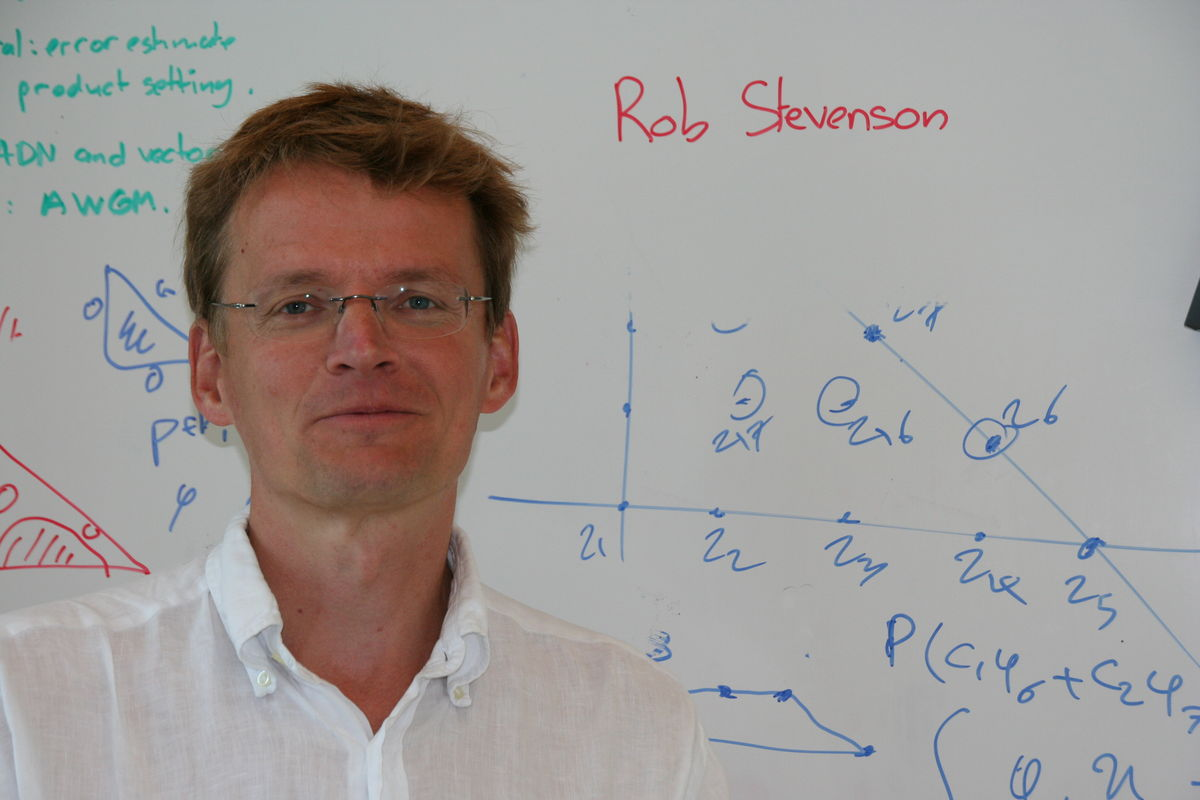
\includegraphics[width=\linewidth]{robbierobrob.jpg}
    \end{column}
  \end{columns}
}

\frame{
  \frametitle{Fourier Transformatie (Recap)}
  \begin{columns}
    \begin{column}{0.75\linewidth}
      \[ \left\{ e^{i k 2 \pi x}: k \in \mathbb{N}_0 \right\} \]
      \[ f = \sum \langle f, \phi_k \rangle \phi_k\text{, met $\phi_k$ genormaliseerd } \]

      \begin{itemize}
      \item Functie schrijven in de Fourier-basis
      \item co\"efficienten kleiner dan $\epsilon$``weggooien"
      \item signaal reconstrueren adhv kleinere set co\"efficienten
      \end{itemize}
    \end{column}
    \begin{column}{0.25\linewidth}
      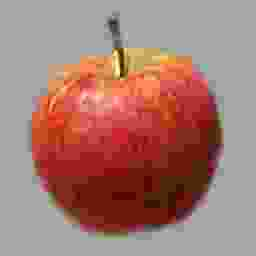
\includegraphics[width=\linewidth]{Sample2.jpg}
    \end{column}
  \end{columns}
}

\section{Wavelets}

\frame{
  \frametitle{Wavelet Transformatie}
  \begin{columns}
    \begin{column}{0.4\linewidth}
      %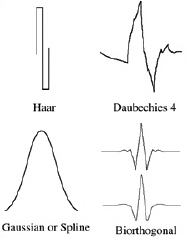
\includegraphics[width=\linewidth]{4wavelets.jpg}
    \end{column}
    \begin{column}{0.6\linewidth}
      \begin{itemize}
      \item Weer othonormale basis
      \item Kleinere drager $\implies$ discontinuiteiten alleen locaal zichtbaar
      \item Vari\"eteit aan families en klassen
      \item Schalingsfunctie $\phi_\lambda$ en Waveletfunctie $\psi_\lambda$
      \end{itemize}
    \end{column}
  \end{columns}
}

\frame{
  \frametitle{Haarwavelet / Daubechies Wavelet}
  \begin{itemize}
    \item Simpelste Wavelet
    \item Schalings en wavelet functie oder watever
    \item 
  \end{itemize}
}

\frame{
  \frametitle{Wavelet Transformatie}
  \begin{itemize}
    \item Discrete functie van lengte $N = 2^n$
    \item op zoek naar $\langle f, \psi_\lambda \rangle$
    \item $f \in V_n$ met $V_n$ ruimte van stuksgewijs constante functies op $2^n$ segmenten (dus $V_0 \subset V_1 \subset \ldots$)
    \item Bouw $W_i \perp V_i$ zo dat $V_{i+1} = V_i \oplus W_i \implies V_n = V_0 \oplus W_0 \oplus \ldots \oplus W_{n-1}$
    \item Per constructie $V_i = span\{\phi_{i,n} : n \in \mathbb{Z}\}$
  \end{itemize}
}

\frame{
  \frametitle{Voorbeeld met Haar}
  \begin{columns}
    \begin{column}{0.5\linewidth}
      Hier moet plaatje bij van wavelet.\\
      De Haarwavelet heeft filters:
      \begin{itemize}
      \item $h = \frac 1 2 \sqrt 2 \cdot (-1,1)$
      \item $g = \frac 1 2 \sqrt 2 \cdot (1,1)$
      \end{itemize}
      Signaal : $a_0 = (1,2,1,2,3,4,3,4)$ \\ 
      
      $a_1 = \frac 1 2 \sqrt 2 \cdot (3,3,7,7)$
      $d_1 = \frac 1 2 \sqrt 2 \cdot (-1,-1,-1,-1)$
      
      $a_2 = (3,7)$
      $d_2 = (0,0)$

      $a_3 = \frac12\sqrt2\cdot (10)$
      $d_3 = \frac12\sqrt2\cdot (-4)$
      \end{column}
    \begin{column}{0.5\linewidth}
      \centering (Kijk hier naar)
      \begin{eqnarray*}
        a_{i+1}[n] = \sum_k h[k-2n]a_j[k] \\
        d_{i+1}[n] = \sum_k g[k-2n]a_j[k] 
      \end{eqnarray*}
    \end{column}
  \end{columns}

  Uiteindelijk getransformeerde wordt:
  $\frac12\sqrt2\cdot(10,-4,0,0,-1,-1,-1,-1)$
}

\section{Plaatjes}

\frame{
  \frametitle{LoodRecht (Plaatjes)}
  (mallacdecompositie.jpg)
  \begin{itemize}
    \item Generalisering naar meer dimensies
    \item Mallat-decompositie.txt
    \item 
  \end{itemize}
}

\frame{
  \frametitle{Voorbeelden}
  Hier komen: Gentoo op verschillende compressie niveau's met FFT / Haar / DB2
}

\section{Filmpjes}

\frame{
  \frametitle{Filmpjes $\implies$ 3D signaal}
  \begin{itemize}
    \item Natuurlijke voortzetting van Mallat-decompositie
    \item Voorbeeldtjes
  \end{itemize}
}

\frame{
  \frametitle{Maar toen...}
  vergelijkingMallat-vs-Tensor.jpg
  \begin{itemize}
    \item Vermoeden van Rob over filmpjes
    \item Tensor decompositie i.p.v. Mallat decompositie
    \item HTML magicks
  \end{itemize}
}

\section{Wat nu?}

\frame{
  \frametitle{Inhoudsopgave}
  \itemize{

  \item Deel over Fourier

    \itemize{
    \item[-] Analyse van Discrete Fourier Transform
    \item[-] Fast Fourier Transform algoritme
    \item[-] Toepassing van FFT op plaatjes/geluid w/e
    }

  \item Deel over Wavelets

    \itemize{
    \item[-] Theoretische beschouwing van wavelets
    \item[-] Toepassing van Wavelets $\implies$ DWT
    \item[-] Analyse van de DWT
    \item[-] Toepassing van DWT op plaatjes/geluid
    \item[-] Tensor product en filmpjes
    }

  \item Vergelijkend deel Wavelets vs. Fourier + Results
  }
}

\frame{
  \frametitle{Wat nog moet gebeuren}
  \itemize{
    \item Kijken naar convergentie eigenschappen van de fout
    \item Afronden van wat we nu hebben
    \item Eventueel nog iets interessants onderzoeken
    \item Code opschonen
  }
}

\end{document}
